     \documentclass[xcolor=dvipsnames, 9pt]{beamer}
     \usepackage{fancyhdr, amsmath, amsthm, amssymb, mathtools, lastpage,
     hyperref, enumerate, graphicx, setspace, wasysym, upgreek, listings, times}
     \usetheme{Madrid}
     \usefonttheme{professionalfonts}
     \newcommand{\scinot}[2]{#1\times10^{#2}}
     \newcommand{\bra}[1]{\left<#1\right|}
     \newcommand{\ket}[1]{\left|#1\right>}
     \newcommand{\dotp}[2]{\left<#1\,\middle|\,#2\right>}
     \newcommand{\rd}[2]{\frac{\mathrm{d}#1}{\mathrm{d}#2}}
     \newcommand{\pd}[2]{\frac{\partial#1}{\partial#2}}
     \newcommand{\rtd}[2]{\frac{\mathrm{d}^2#1}{\mathrm{d}#2^2}}
     \newcommand{\ptd}[2]{\frac{\partial^2 #1}{\partial#2^2}}
     \newcommand{\norm}[1]{\left|\left|#1\right|\right|}
     \newcommand{\abs}[1]{\left|#1\right|}
     \newcommand{\pvec}[1]{\vec{#1}^{\,\prime}}
     \newcommand{\svec}[1]{\vec{#1}\;\!}
     \newcommand{\bm}[1]{\boldsymbol{\mathbf{#1}}}
     \let\Re\undefined
     \let\Im\undefined
     \newcommand{\ang}[0]{\text{\AA}}
     \newcommand{\mum}[0]{\upmu \mathrm{m}}
     \DeclareMathOperator{\Res}{Res}
     \DeclareMathOperator{\Re}{Re}
     \DeclareMathOperator{\Im}{Im}
     \DeclareMathOperator{\Log}{Log}
     \DeclareMathOperator{\Arg}{Arg}
     \DeclareMathOperator{\Tr}{Tr}
     \DeclareMathOperator{\E}{E}
     \DeclareMathOperator{\Var}{Var}
     \DeclareMathOperator*{\argmin}{argmin}
     \DeclareMathOperator*{\argmax}{argmax}
     \DeclareMathOperator{\sgn}{sgn}
     \DeclareMathOperator{\diag}{diag}
     \newcommand{\expvalue}[1]{\left<#1\right>}
     \usepackage[labelfont=bf, font=scriptsize]{caption}\usepackage{tikz}
     \usepackage[font=scriptsize]{subcaption}
     \everymath{\displaystyle}
     \lstset{basicstyle=\ttfamily\footnotesize,frame=single,numbers=left}
\tikzstyle{circ} = [draw, circle, fill=white, node distance=3cm, minimum
height=2em]

\title[MongoDB World 2017]{Blend in Chicago: MongoDB World 2017}
% \subtitle[]{Subtitle}
\author[Y. Su]{Yubo Su}
\institute[Blend]{Blend}
\date{\today}
\logo{%
    \makebox[0.95\paperwidth]{%
        
\includegraphics[width=0.15\textwidth]{media/mongo.png}
        \hfill
        
\includegraphics[width=0.15\textwidth]{media/blend.png}
    }
}
\setbeamertemplate{caption}{\insertcaption\par}

\begin{document}

\frame{\titlepage}

\begin{frame}
    \frametitle{Morning Keynotes}
    \framesubtitle{06/20/17 0900--1030}

    \begin{itemize}
        \item Tom Schenk, Chief data officer, Chicago. \emph{WindyGrid}.
            \begin{itemize}
                \item Track colocated data, 911 calls to Tweets to
                    weather.
                \item Flexible schema: \texttt{\{what, when, where\}}
                \item Predictive analytics (example, where to send food
                    inspector) using visualization of multiple causal layers.
            \end{itemize}
        \item Dev Ittycheria, CEO MongoDB
            \begin{itemize}
                \item 2007 is watershed year, AWS, iPhone, Android, and
                    many others.
                \item Argue b/c storage costs dropped below a critical
                    point.
                \item MongoDB also in 2007: document model, distributed
                    systems + aggregation.
            \end{itemize}
    \end{itemize}
\end{frame}

\begin{frame}
    \frametitle{Morning Keynotes}
    \framesubtitle{06/20/17 0900--1030}
    \begin{itemize}
        \item Eliot Horowitz, CTO, MongoDB
            \begin{itemize}
                \item 3.6 ships November, already on Github.
                \item MongoDB Charts (3.6)
                    \begin{itemize}
                        \item Business Intelligence: BI Connector is SQL
                            interface.
                        \item Coercing data to table is difficult:
                            polymorphic schemas, arrays.
                        \item Solution: \emph{MongoDB Charts}! Data
                            visualization tool, handles above.
                    \end{itemize}

                \item 3.6 document model features:
                    \begin{itemize}
                        \item \texttt{\$lookup} takes sub-pipelines!
                        \item \texttt{\$update} can operate on arrays
                            natively! Takes a filter over array entries,
                            can iterate over nested.
                        \item JSON Schemas.
                    \end{itemize}

                \item 3.6 distributed systems:
                    \begin{itemize}
                        \item Native retryable writes
                        \item \emph{Change Streams} can get a stream of changes
                            to a db.
                    \end{itemize}
            \end{itemize}
    \end{itemize}
\end{frame}

\begin{frame}
    \frametitle{Morning Keynotes}
    \framesubtitle{06/20/17 0900--1030}
    \begin{itemize}
        \item Eliot Horowitz, CTO, MongoDB (continued)
            \begin{itemize}
                \item Mongo Atlas
                    \begin{itemize}
                        \item ``Should be irrespensible to run MongoDB in cloud
                            w/o Atlas''
                        \item Built in security, one-click spin up, built in
                            scaling elasticity.
                        \item Data browser + performance viewer in UI
                            (utilization stats, examine queries as stream,
                            explore data),
                        \item Live migration service (not very live in demo,
                            requires downtime for mirror to catch up and change
                            source of truth).
                        \item Now with MS Azure + Google Cloud support too (+
                            AWS). \\[9pt]
                        \item Performance Adviser.
                        \item CRUD support in data browser.
                        \item Charts!
                        \item LDAP Auth.
                        \item Cross-region, cross-cloud!
                    \end{itemize}
                \item MongoDB Stich (Beta as of today in Atlas, 06/20/17)
                    \begin{itemize}
                        \item ``Backend as a service''
                        \item REST API for MongoDB
                        \item Configuration-based auth/security
                        \item Service composition to govern how services talk to
                            each other.
                    \end{itemize}
            \end{itemize}
    \end{itemize}
\end{frame}

\begin{frame}
    \frametitle{Squeezing the Most out of Your Document Model}
    \framesubtitle{%
        06/20/17 1050--1130:
        Norberto Leite, Lead Curriculum Engineer, MongoDB
    }
    \begin{columns}
        \begin{column}{0.5\textwidth}
            \begin{itemize}
                \item Nested schema, spectrum of highly normalized or denormed storage.
                    \begin{itemize}
                        \item Normalized requires foreign keys, requires looking
                            into many collections.
                        \item Denorm is simpler query, complex schema.
                    \end{itemize}
                \item Consider three possible behaviors:
                    \begin{itemize}
                        \item Get player: Denorm outperforms.
                        \item Add new field to doc: either add new collection
                            or modify every doc, the same.
                        \item Change existing field: If a highly shared field,
                            normalized is very fast.
                    \end{itemize}
            \end{itemize}
        \end{column}
        \begin{column}{0.5\textwidth}
            \begin{itemize}
                \item Optimizing highly normalized:
                    \begin{itemize}
                        \item Can optimize with aggregate, but more importantly
                            \texttt{db.createView()}.
                            \begin{itemize}
                                \item Views are basically stored aggregates.
                                \item Better \texttt{\$project} support.
                            \end{itemize}
                        \item Also consider, if reading much more than writing,
                            should store calculated fields!
                    \end{itemize}
                \item Optimizing denormed:
                    \begin{itemize}
                        \item Should normalize fields that are infrequently
                            updated.
                    \end{itemize}
                \item \texttt{tl;dr} normalized have fast write, slow reads.
                    Should embed everything that is infrequently updated.
            \end{itemize}
        \end{column}
    \end{columns}
\end{frame}

\begin{frame}
    \frametitle{Advanced Schema Design Patterns}
    \framesubtitle{%
        06/20/17 1140--1220:
        Daniel Coupal, Senior Curriculum Engineer, MongoDB
    }
    \begin{columns}
        \begin{column}{0.5\textwidth}
            \begin{itemize}
                \item Axiom: data models maximize performance + scalability
                    despite latency, costs, hardware.
                \item Common issues \#1, too many optional fields:
                    \begin{itemize}
                        \item Use attribute array, \texttt{[\{key: keyName, value\}]}.
                        \item Accommodates optional fields.
                    \end{itemize}
                \item Common issues \#2, working set does not fit in RAM.%
                    \begin{itemize}
                        \item Can subset, truncate data
                        \item Probably also useful for showing users too.
                    \end{itemize}
                \item Common issues \#3, data consistency.
                    \begin{itemize}
                        \item Accept instantaneous inconsistency, duplicate at
                            regular intervals \frownie.
                    \end{itemize}
            \end{itemize}
        \end{column}
        \begin{column}{0.5\textwidth}
            \begin{itemize}
                \item Common issues \#4, repeated computations
                    \begin{itemize}
                        \item Reads generally outnumber writes, apply
                            computation on write.
                    \end{itemize}
                \item Common issues \#5, expensive tracking
                    \begin{itemize}
                        \item e.g.\ expensive to increment on every page view
                        \item Solution: random number in range $[1, N]$,
                            increment by $N$.
                    \end{itemize}
                \item Common issues \#6, large data easily overflow
                    \begin{itemize}
                        \item Bucket, store buckets into a separate
                            collection.
                    \end{itemize}
            \end{itemize}
        \end{column}
    \end{columns}
\end{frame}

\begin{frame}
    \frametitle{Powering Microservices with Docker, Kubernetes, Kafka and MongoDB}
    \framesubtitle{%
        06/20/17 1350--1430:
        Andrew Morgan, Product Marketing, MongoDB
    }
    \begin{itemize}
        \item Microservices vs.\ monolith, preferable b/c web scale,
            faster iteration, compartmentalized.
        \item One common rule of thumb is that one developer can own the
            whole thing, a couple hundred lines, but not everybody
        \item Hard metal vs.\ Docker (Kubernetes) vs.\ Atlas.
        \item Kafka can run general events while Mongo streams (the new feature)
            only handles database updates.
    \end{itemize}
\end{frame}

\begin{frame}
    \frametitle{Index Usage for Nested Logical Queries}
    \framesubtitle{%
        06/20/17 1440--1520:
        Tess Avitabile, Software engineer, MongoDB
    }
    \begin{columns}
        \begin{column}{0.5\textwidth}
            \begin{itemize}
                \item Query system overview:
                    \begin{itemize}
                        \item Input: JSON
                        \item Parse into tree
                        \item Generate plan (which indicies for which leaves of
                            the tree)
                        \item Plan selection: try all of the plans for a trial
                            period, see which one was fastest (Note: plan
                            caching)
                        \item Execution \& return
                    \end{itemize}
                \item \texttt{OR}s inside of \texttt{AND}s is a pain for plan
                    generation.
                    \begin{itemize}
                        \item \texttt{AND} is considered indexed when one child
                            has index.
                        \item \texttt{OR} is considered indexed when all
                            children have indicies.
                        \item \texttt{OR}s have to dedupe by hashing to merge
                            the two results.
                    \end{itemize}
            \end{itemize}
        \end{column}
        \begin{column}{0.5\textwidth}
            \begin{itemize}
                \item Problem: no tight index bounds on these queries
                    \begin{itemize}
                        \item \emph{Tight} index bounds are when all documens in
                            index bounds match the query.
                        \item (As opposed to when a parent node imposes a
                            filter, \texttt{FETCH})
                    \end{itemize}
                \item Bounds are not tight b/c two branches of children cannot
                    talk to each other! e.g.\ the \texttt{OR} will not be tight
                    since the \texttt{AND} above will have to further fetch
                    against its other child.
            \end{itemize}
        \end{column}
    \end{columns}
\end{frame}

\begin{frame}
    \frametitle{Index Usage for Nested Logical Queries (cont)}
    \framesubtitle{%
        06/20/17 1440--1520:
        Tess Avitabile, Software engineer, MongoDB
    }
    \begin{columns}
        \begin{column}{0.5\textwidth}
            \begin{itemize}
                \item Solution: Disjunctive Normal Form?
                    \begin{itemize}
                        \item \texttt{AND} with \texttt{OR} child solved!
                        \item Exponentially many plans though, index choices at
                            each child.
                    \end{itemize}
                \item Solution: OR-pushdowns! Predicates pulled up to the
                    \texttt{AND} parent and pushed down into any \texttt{OR}
                    children if they can tighten index bounds.
                    \begin{itemize}
                        \item Note that this is not imposed as an extra
                            \texttt{AND} condition, just metadata for the
                            recursive query planner to plan against.
                    \end{itemize}
                \item Paper: Query Optimization by Predicate Move-Around
            \end{itemize}
        \end{column}
        \begin{column}{0.5\textwidth}
            \begin{figure}[!h]
                \centering
                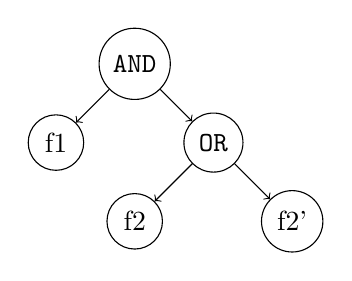
\begin{tikzpicture}
                    \node[circ, radius=0.2] (and) at (0, 0) {\texttt{AND}};
                    \node[circ, radius=0.2] (f1) at (-1, -1) {f1};
                    \node[circ, radius=0.2] (or) at (1, -1) {\texttt{OR}};
                    \node[circ, radius=0.2] (f2) at (0, -2) {f2};
                    \node[circ, radius=0.2] (f3) at (2, -2) {f2'};
                    \draw[->] (and)--(or);
                    \draw[->] (and)--(f1);
                    \draw[->] (or)--(f2);
                    \draw[->] (or)--(f3);
                \end{tikzpicture}
                \caption{\texttt{AND} with \texttt{OR} child. Consider if index
                is \texttt{\{f1, f2\}}? \texttt{\{f2, f1\}}?\label{fig:and_or}}
            \end{figure}
        \end{column}
    \end{columns}
\end{frame}

\begin{frame}
    \frametitle{Multi-Master architectures in MongoDB}
    \framesubtitle{%
        06/20/17 1530--1610:
        Pavel Duchovny, TSE, MongoDB
    }
    \begin{columns}
        \begin{column}{0.5\textwidth}
            \begin{itemize}
                \item Key to geograhpic colocation.
                \item Zone sharding + replica sets
                    \begin{itemize}
                        \item Zone sharding: shards per region.
                        \item Replica sets are \texttt{mongod} processes that
                            share the same data.
                    \end{itemize}
                \item Configuration is:
                    \begin{itemize}
                        \item One primary in each region, each a separate zone
                            shard.
                        \item One secondary in its own region (prio 3), two in
                            another (prio 2), and two more in a third (prio 1,
                            0) for symmetry across all regions, hidden
                            secondary.
                        \item Spread across multiple regions, odd number of
                            voting members, primary DC members should have
                            higher priorities.
                    \end{itemize}
            \end{itemize}
        \end{column}
        \begin{column}{0.5\textwidth}
            \begin{itemize}
                \item Can specify region on read/write.
                \item Upshot is that can do multi-region writes while
                    guaranteeing local availability on read.
                \item Configurable to write to secondary especially if primary
                    lives in a different region.
                \item Can configure with \texttt{MAX\_STALENESS} parameter for
                    when a cluster can be read from.
            \end{itemize}
        \end{column}
    \end{columns}
\end{frame}

\begin{frame}
    \frametitle{Globally Distributed RESTful Object Storage}
    \framesubtitle{%
        06/20/17 1620--1700:
        Julio Viera, Backend VP, Fuze
    }
    \begin{columns}
        \begin{column}{0.5\textwidth}
            \begin{itemize}
                \item Built an object store for internal communications, chat +
                    attachment retention, Mongo backbone.
                \item RESTful so easy to expose HTTP link as a db.
                \item Nested schema corresponding to URL:\@
                    {\small\texttt{/users/:id/chat/convs/X/messages/Y}}
                \item Storage (chat), collection (convs), sub-collection
                    (messages), documentIds
            \end{itemize}
        \end{column}
        \begin{column}{0.5\textwidth}
            \begin{itemize}
                \item Pubsub (user is online) can be done by consuming the oplog
                    on the db primary.
                \item To shard and hide it to the user, just need some lookups
                    userId $\to$ sharding keys.
            \end{itemize}
        \end{column}
    \end{columns}
\end{frame}

\begin{frame}
    \frametitle{Evening Keynotes}
    \framesubtitle{06/20/17 1715--1845}

    \begin{itemize}
        \item Saska Mojsilovic, IBM
            \begin{itemize}
                \item Need for more data in health for precision health
                    service distribution.
                \item All sorts of orgs estimating and predicting from
                    sparse data.
            \end{itemize}
        \item Claudio Gosiker (Florida Blue) \& Alan Chhabra (MongoDB)
            \begin{itemize}
                \item Use data for healthcare outreach, personalizable
                    views for customer reps.
            \end{itemize}
        \item Matt Parker, Stand-up Mathematician!
    \end{itemize}
\end{frame}

\begin{frame}
    \frametitle{Morning Keynotes}
    \framesubtitle{06/21/17 0900--1030}

    \begin{columns}
        \begin{column}{0.5\textwidth}
            \begin{itemize}
                \item Bjorn Freeman-Benson, CTO, InVisionApp
                    \begin{itemize}
                        \item Via microservices, can stand up new cluster in 10m!
                        \item Also has a \texttt{bailey stage it} etc.
                        \item QA against EA customers, automatically rolls out to rest
                            of customers afterwards (24h).
                    \end{itemize}
                \item Cisco moved eCommerce to MongoDB, 40b connections?
                \item Justin Moses, Lead Software Engineer, MongoDB
                    \begin{itemize}
                        \item Data auralization vs.\ visualization!
                        \item \href
                            {https://www.npmjs.com/package/node-keyboard}
                            {\texttt{npmjs link}}
                        \item Just turns numbers into music.
                    \end{itemize}
            \end{itemize}
        \end{column}
        \begin{column}{0.5\textwidth}
            \begin{itemize}
                \item Jane McGonigal, Game Designer, AvantGame
                    \begin{itemize}
                        \item 2.1b gamers $>$ 1h/day, more stats.
                        \item 72\% workforce not engaged, vs.\ 80+\% of
                            schoolchildren engaged.
                        \item Consider: \emph{``Opposite of play is not work but
                            depression.''}
                        \item Video games overstimulate brain regions exactly
                            what depression supresses.
                        \item Pokemon Go fitness lol.
                        \item Reality's obligation to engage the way video games
                            do, AR $>$ VR!%
                    \end{itemize}
            \end{itemize}
        \end{column}
    \end{columns}
\end{frame}

\begin{frame}
    \frametitle{Migrating from EC2 to Atlas}
    \framesubtitle{%
        06/20/17 1050--1130:
        Jesse Dearing, SRE, InVision
    }
    \begin{columns}
        \begin{column}{0.5\textwidth}
            \begin{itemize}
                \item Mongo at InVision
                    \begin{itemize}
                        \item 28 replica sets 4 env
                        \item 2000 rps, 600 wps
                        \item Chef to manage EC2, Mongo
                    \end{itemize}
                \item Old stack:
                    \begin{itemize}
                        \item EC2 instance, deploy, manually configure/shard
                        \item Manual: backups, monitoring, alerting, security, updates
                    \end{itemize}
                \item Atlas:
                    \begin{itemize}
                        \item All above, REST API, dashboards
                    \end{itemize}
                \item Transition Preparation
                    \begin{itemize}
                        \item SSL (Atlas mandatory)
                        \item AWS VPC Peering
                        \item VPN + security setup, Amazon DNS
                        \item MongoDB 3.x + WiredTiger
                    \end{itemize}
            \end{itemize}
        \end{column}
        \begin{column}{0.5\textwidth}
            \begin{itemize}
                \item Transition
                    \begin{itemize}
                        \item UI Live Migrator ($<$1m downtime for oplog)
                        \item \texttt{mongomirror} for full ZDT:\@ Initial sync,
                            streams oplog, point to new instance \emph{before}
                            fully synced, continues syncing.
                        \item Full ZDT but momentary inconsistency ($<$ 1s).
                        \item In case of rolling ZDT deploys when re-pointing,
                            inconsistency is most noticable; graceful
                            degredation!
                    \end{itemize}
                \item Epilogue
                    \begin{itemize}
                        \item Alerts, new playbooks, backup restores.
                        \item Automatic provisioning for new services that need
                            MongoDB.%
                    \end{itemize}
            \end{itemize}
        \end{column}
    \end{columns}
\end{frame}

\end{document}
